% !TEX encoding = UTF-8
% !TEX TS-program = pdflatex
% !TEX root = ../../tesi.tex

\section{Vincoli metodologici}
Durante il percorso di stage ho configurato quattro \textit{repository}: \textit{smart contract} per Ethereum, \textit{smart contract} per HotMoka, la libreria per la comunicazione del \textit{back-end} con gli \textit{smart contract} precedentemente elencati e lo \textit{standard ERC721} per HotMoka. Per ognuna di queste ho applicato uno specifico \textit{Way Of Working} che verrà spiegato di seguito. \\

Inizialmente, come la metodologia Scrum vuole, è stato definito per ogni prodotto il proprio \textbf{\textit{product backlog}} attraverso la creazione delle varie \textit{issue}. In seguito, sono state associate ad una \textit{milestone}, prefissata con il mio \textit{tutor} aziendale, Fabio Pallaro, ed alla relativa \textit{board}, così da poterle gestire avendo una visione migliore delle attività da fare, quelle in progresso e quelle completate.

\clearpage
\begin{figure}[h!]
  \centering
  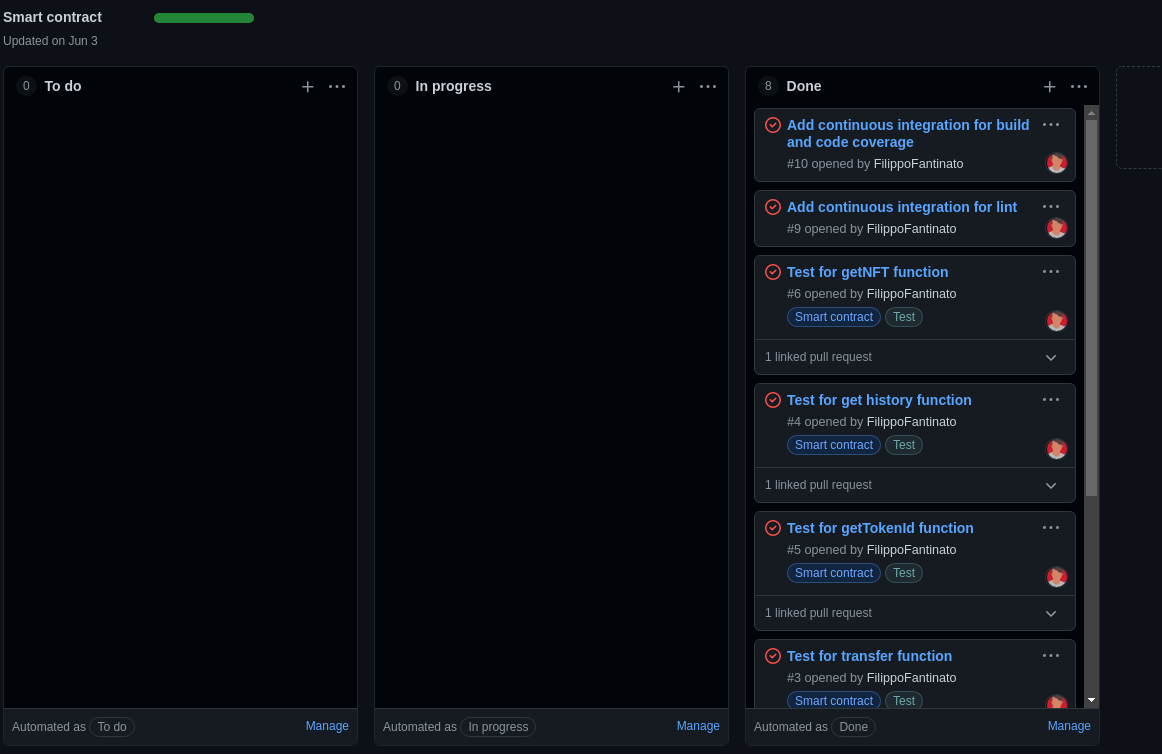
\includegraphics[width=0.8\textwidth]{capitolo3/smart-contract-ethereum-board.png}
  \caption{Esempio di utilizzo della \textit{board}}
  \textbf{Fonte}: \href{https://github.com/NFT-Lab/smart-contract-ethereum/projects/1}{https://github.com/NFT-Lab/smart-contract-ethereum/projects/1}
\end{figure}

Durante lo svolgimento dello \textit{sprint}, quando una \textit{issue} cambia il suo stato in progresso, viene \textbf{aperto un nuovo \textit{branch}} legato ad essa, dove viene implementata la nuova funzionalità.

Al termine dell'implementazione della funzionalità, viene creata una \textbf{\textit{pull request}}, la quale avvia la \textit{action} che esegue l'analisi statica e i vari test automatici che sono stati programmati. In questo modo viene verificata la validità del codice che si vuole integrare con quello già presente nel \textit{branch develop}. Una volta approvata la \textit{pull request} e avvenuta la fusione tra il codice presente nel \textit{feature branch} e quello nel \textit{develop}, viene eseguita un'altra \textit{action} che ha lo stesso compito di quella precedente, ma in più andrà ad eseguire il \textit{report} del \textit{code coverage} raggiunto al servizio \textit{Coveralls}.

% \clearpage
\begin{figure}[h!]
  \centering
  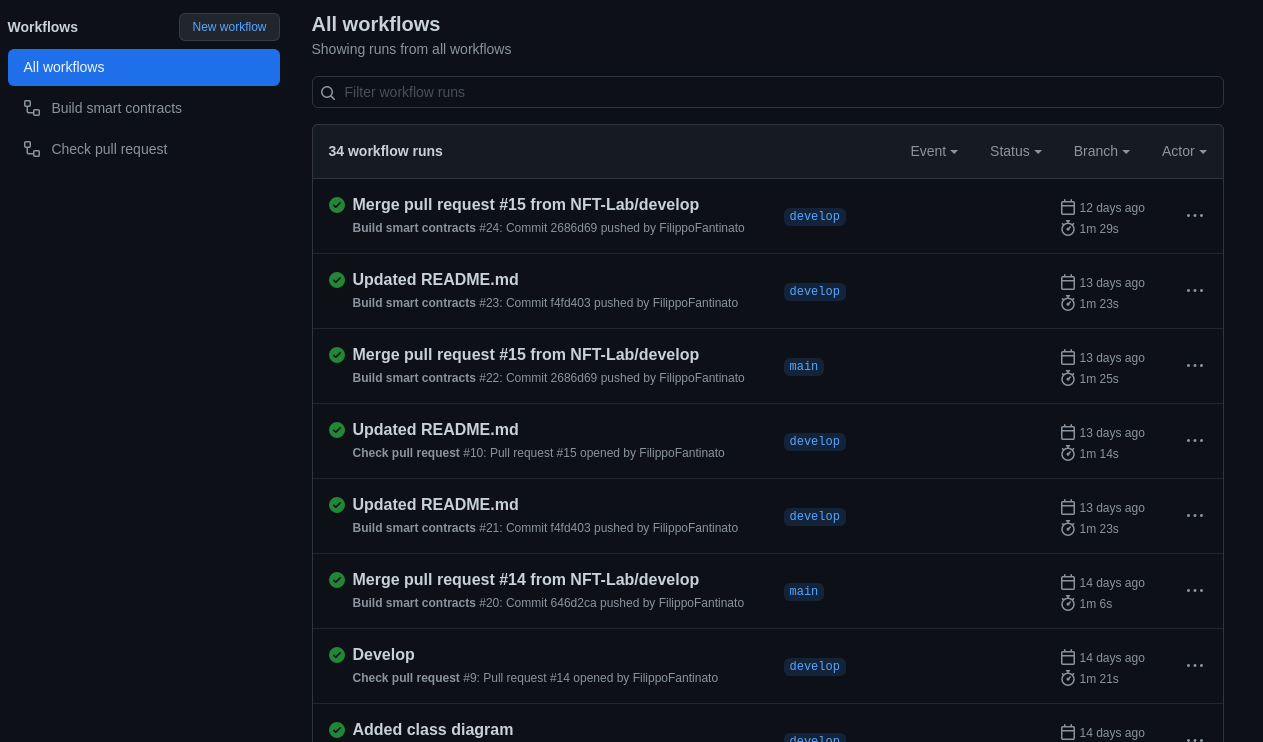
\includegraphics[width=0.9\textwidth]{capitolo3/smart-contract-ethereum-actions.png}
  \caption{Pagina di GitHub \textit{Action} dello \textit{smart contract} per Ethereum}
  \textbf{Fonte}: \href{https://github.com/NFT-Lab/smart-contract-ethereum/actions}{https://github.com/NFT-Lab/smart-contract-ethereum/actions}
\end{figure}

\begin{figure}[h!]
  \centering
  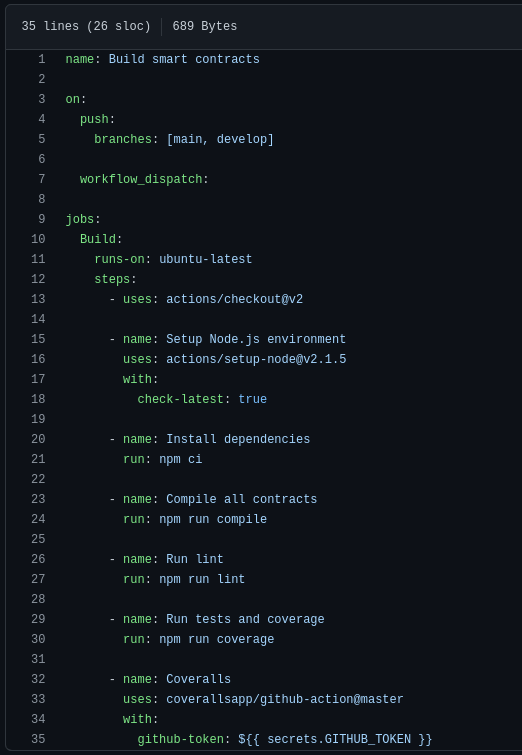
\includegraphics[width=0.9\textwidth]{capitolo3/smart-contract-ethereum-build-action.png}
  \caption{\textit{Action} che esegue la build dello \textit{smart contract} per Ethereum}
  \textbf{Fonte}: \href{https://github.com/NFT-Lab/smart-contract-ethereum/blob/main/.github/workflows/build.yml}{build.yml}
\end{figure}

Quando tutte le \textit{issue} relative ad una \textit{milestone} sono state chiuse, è possibile iniziare la \textbf{\textit{release}}. Viene creato un \textit{branch} di tipo \textit{release} e, dopo aver effettuato degli eventuali \textit{bugfix}, viene avviata una \textit{pull request} da questo \textit{branch} verso il \textit{branch main} e \textit{develop}. Viene verificato, come nel caso di altre \textit{pull request}, la validità del codice che deve essere integrato. In seguito all'approvazione delle \textit{pull request}, viene aggiunto il codice e creata la release attraverso la dichiarazione di un nuovo \textit{tag}. In questo momento vengono avviate due \textit{action}: quella che va a verificare la validità del codice presente nel \textit{branch main} e \textit{develop}, eseguendo l'analisi statica del codice, i test automatici e il report del \textit{code coverage} raggiunto al servizio \textit{Coveralls}, e quella che ha il compito di pubblicare sul \textit{artifact repository} di GitHub il pacchetto generato dalla fase di build.

\begin{figure}[h!]
  \centering
  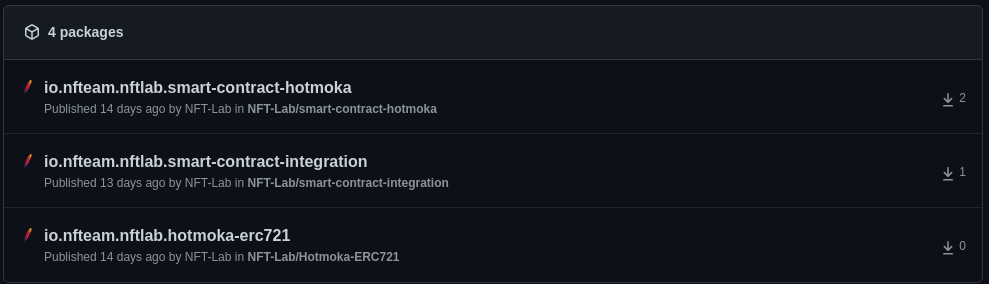
\includegraphics[width=0.9\textwidth]{capitolo3/nftlab-artifact-repository.png}
  \caption{\textit{Artifact repository} dell'organizzazione NFTLab}
  \textbf{Fonte}: \href{https://github.com/orgs/NFT-Lab/packages}{https://github.com/orgs/NFT-Lab/packages}
\end{figure}
